\documentclass[a4paper, twoside, 12pt]{report}

\usepackage{titlesec}
\usepackage{polski}
\usepackage[english, polish]{babel}
\usepackage{graphicx}
\usepackage[hidelinks]{hyperref}
\usepackage{pdfpages}
\graphicspath{ {./images/} }
\usepackage[utf8]{inputenc}
\usepackage[margin=25mm]{geometry}
\usepackage{indentfirst}
\linespread{1}
\titleformat*{\section}{\fontsize{14pt}{2}\bfseries}
\titleformat*{\subsection}{\fontsize{13pt}{2}\bfseries}
\titleformat*{\subsubsection}{\fontsize{13pt}{2}\bfseries}
\usepackage[T1]{fontenc}
% \usepackage{tgtermes}

\newenvironment{abstractpage}
  {\vspace*{\fill}\thispagestyle{empty}}
    {\vfill}
    \renewenvironment{abstract}[1]
      {\bigskip\selectlanguage{#1}%
             \begin{center}\bfseries\abstractname\end{center}}
           {\par\bigskip}

\begin{document}

% 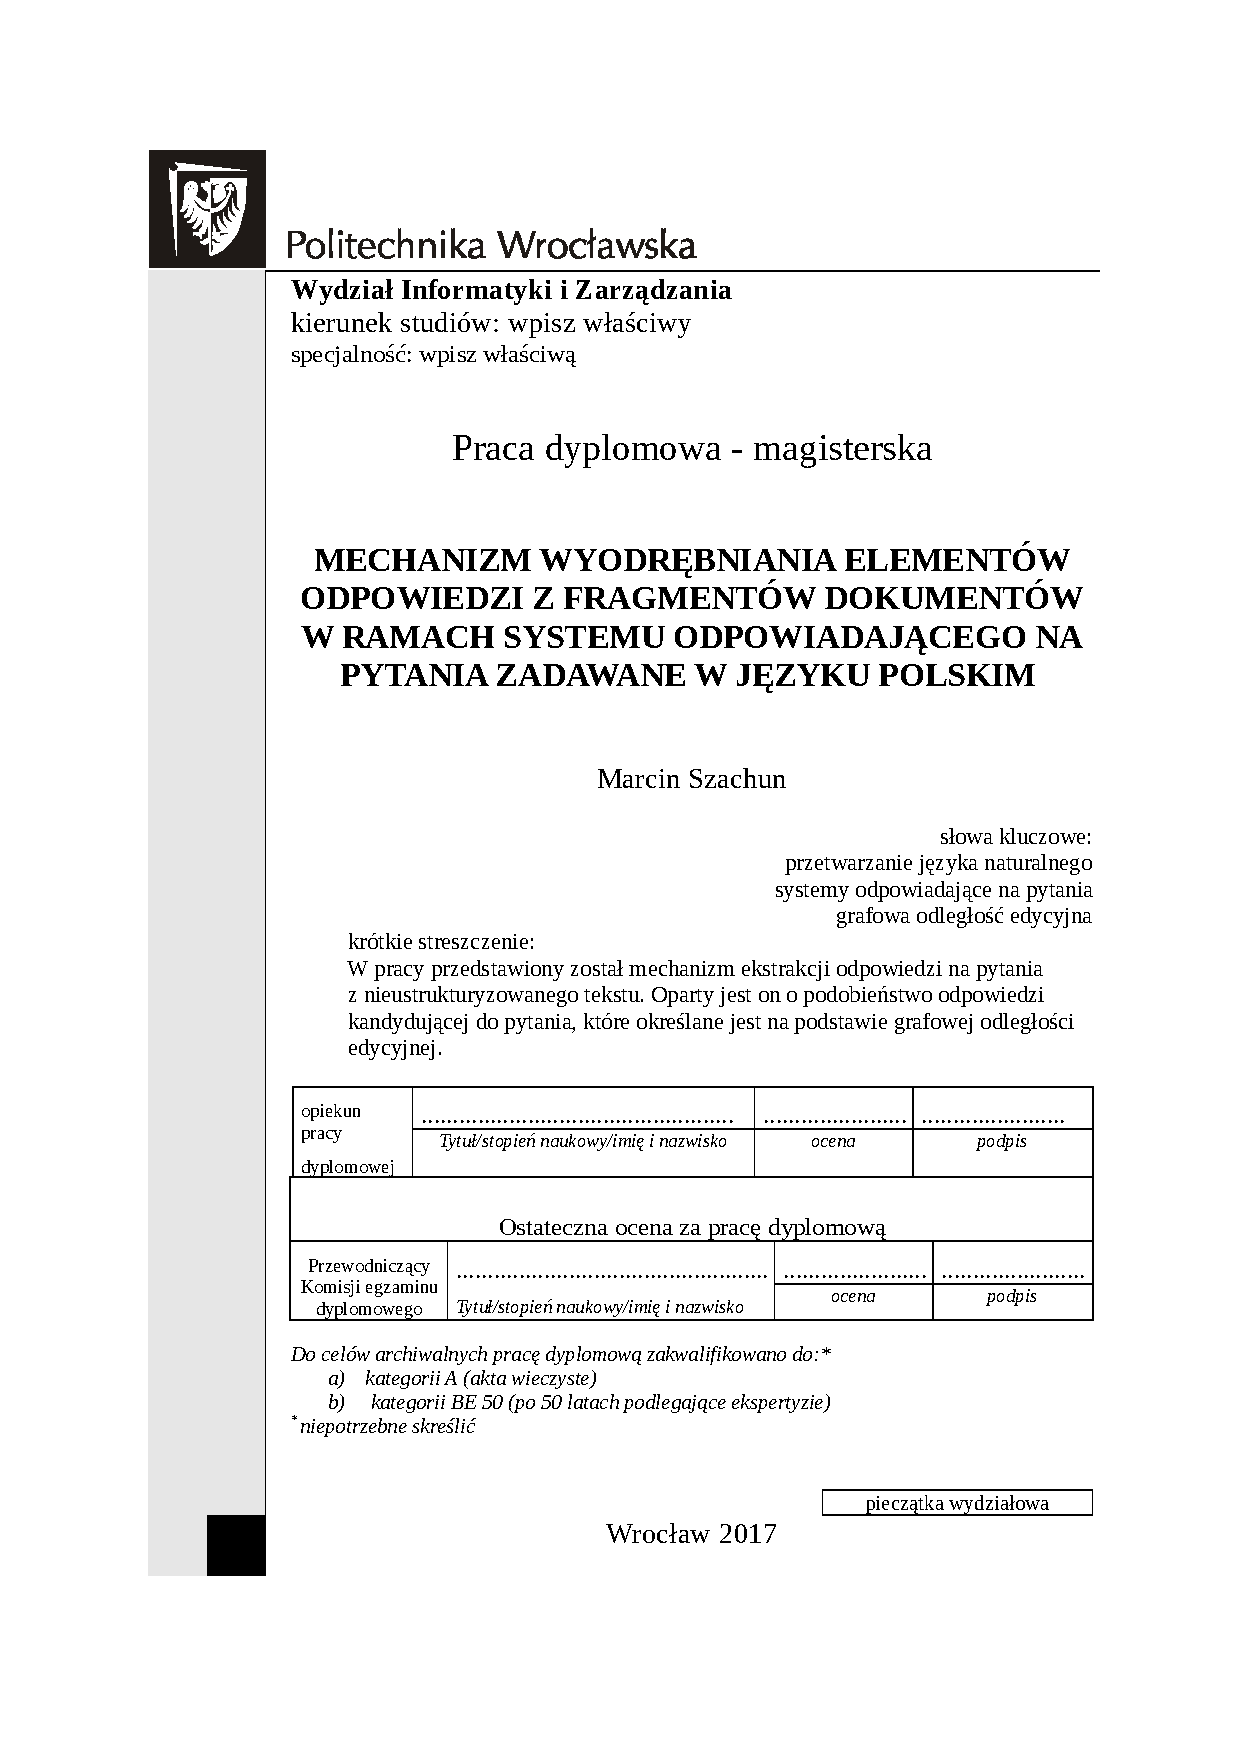
\includepdf{stronatytulowa.pdf}


\begin{abstractpage}
\begin{abstract}{polish}
    W dzisiejszych czasach Internet pełen jest informacji na praktycznie dowolny temat. Wraz ze wzrastającą ilością
    dostępnych informacji, niezmiernie ważne staje się opracowanie mechanizmów pozwalających znaleźć informacje
    interesujące użytkownika. Nie jest to proste, ze względu na to, że informacje te zapisane są najczęściej w formie
    nieustrukturyzowanego tesktu. Tradycyjnie w tym celu wykorzystywane były wyszukiwarki internetowe. Niestety
    języki zapytań używane przez wyszukiwarki internetowe powodują, że wyrażenie precyzyjnej potrzeby informacyjnej
    przez użytkownika jest trudne, a niekiedy niemożliwe. Jednym z proponowanych rozwiązań tego problemu są systemy
    odpowiadające na pytania, w których zapytania formułowane są w formie pytań w języku naturalnym. Niniejsza
    praca zawiera krótkie przedstawienie dziedziny Question Answering, zajmującej się tworzeniem tego typu systemów,
    wraz z opisem systemu ,,Borsuk'' stworzonego na Politechnice Wrocławskiej.
    W głównej części pracy opisana została propozycja nowego mechanizmu ekstrakcji odpowiedzi z fragmentów dokumentów,
    opartego na zmodyfikowanej odległości edycyjnej jako miary podobieństwa między pytaniem a zdaniami mogącymi zawierać
    odpowiedź. Modyfikacja polega na dynamicznym przypisywaniu kosztu operacjom edycji w zależność od słowa. Przeprowadzone
    zostały badania pozwalające optymalnie dobrać wartości tych kosztów. Po zaimplementowaniu tego mechanizmu w systemie "Borsuk",
    wykonane zostały też badania mające na celu porównanie precyzji i dokładności odpowiadania na pytania przed i po
    zastosowaniu opisywanego mechanizmu.
\end{abstract}

\begin{abstract}{english}
    Nowadays the Internet is full of information on almost every topic. With growing amount of available information,
    providing ways to find specific information that user wants is becoming more and more important. Traditionally
    search engines were intended for that purpose. Unfortunately query languages used by search engines are sometimes
    insufficient for expressing user's infomation needs. One of proposed solutions are question answering systems, in which
    queries are formulated using natural language. This thesis contains quick overview of question answering discipline,
    which is concerned with build such systems and description of "Borsuk" system, created by Wrocław University of Technology.
    In main part, new answer extraction mechanism is presented. It is based on using modified tree edit distance as a measure of
    similarity question and sentences that ma contain answer. Modification lies in dynamically assing cost to edit operations
    based on word. Research was conducted to find out optimal cost for operations. Furthermore after implementing this
    mechanism in "Borsuk" question answering system, additional research was conducted to compare precision and accuracy
    of question answering before and after using described mechanism
\end{abstract}
\end{abstractpage}

\tableofcontents

\listoffigures

\chapter{Cel i~zakres pracy}
    Celem niniejszej pracy jest przedstawienie mechanizmu rozszerzającego system odpowiadający na pytania ,,Borsuk''
    pod względem dokładności udzielanych odpowiedzi. Zastosowany mechanizm wykorzystuje odległość edycyjną jako miarę
    podobieństwa między pytaniem a zdaniami zawierającymi odpowiedzi. W~ramach tego celu zostaną wykonane:
    \begin{itemize}
        \item prezentacja i ogólna charakterystyka dziedziny Question Answering wraz z przedstawieniem podstawowych
            pojęć,
        \item opis działania systemów odpowiadających na pytania, wraz z wyróżnieniem poszczególnych faz przetwarznia
            pytania i znajdowania odpowiedzi,
        \item przedstawienie przykładowych, innych niż zaproponowany w~pracy,
            sposobów ekstrakcji odpowiedzi na pytania z fragmentów dokumentów,
        \item zaprezentowanie mechanizmu ekstrakcji odpowiedzi z wykorzystaniem odległości edycyjnej między grafami
            reprezentującymi pytanie oraz zdania kandydujące na odpowiedzi,
        \item przeprowadzenie badań pozwalających na dobranie optymalnych parametrów działania opisywanego
            mechanizmu ekstrakcji odpowiedzi wraz z analizą wniosków z nich płynących,
       \item zaprezentowanie sprawozdania z przebiegu oraz wyników badań porównujących precyzję i dokładność
           odpowiadania na pytania przez system "Borsuk" przed i po implementacji opisanego mechanizmu ekstrakcji
           odpowiedzi.
       \item przeanalizowanie możliwych sposobów kontynuacji prac nad udoskonaleniem przedstawionego mechanizmu

    \end{itemize}

\chapter{Wstęp}
    \section{Przetwarzanie języka naturalnego}
        \subsection{Podstawowe pojęcia}
            \emph{Przetwarzanie języka naturalnego} jest to dziedzina informatyki korzystającą z osiągnięć
            między innymi: sztucznej inteligencji, uczenia maszynowego, nauk kognitywnych
            (zajmujących się obserwacją i~analizą działania ludzkich zmysłów), lingwistyki komputerowej oraz
            wielu innych. Głównym obszarem zainteresowań tej dziedziny jest budowa systemów oraz narzędzi
            umożliwiających wykonywanie użytecznych zadań wiążących się z wykorzystaniem języka naturalnego.
            Obejmuje to zadania takie jak: komunikacja człowiek-komputer, wspomaganie komunikacji międzyludzkiej,
            czy też przetwarzanie tekstu w języku naturalnym bądź mowy\cite{SPEECHANDLANGUAGEPROCESSING}.

            \emph{Język naturalny} jest to język,
            którym posługują się ludzie w codziennej komunikacji między sobą, w sposób naturalny (na przykład
            język polski). Jest to cecha odróżniająca języki naturalne od \emph{języków sztucznych} stworzonych
            do specyficznych zastosowań (na przykład język matematyczny), w tym do komunikacji z komputerem
            (na przykład języki programowania: Assembler, C++, Python).

            Aby umożliwić tworzenie nowych technik
            przetwarzania języka naturalnego oraz ich testowanie niezbędny jest reprezentatywny i zbalansowany
            zbiór tekstów w danym języku. Powinien on zawierać teksty na tyle zróżnicowane, aby pokazać zmienność
            i różne zastosowania języka naturalnego. Przygotowanie takiego zbioru nie wystarczy jednak, aby
            komputer zaczął rozumieć język naturalny. Do tekstów należy dodać metadane, które pozwolą komputerowi
            łatwiej znaleźć wzorce i zależność występujące w danym języku. Jako przykład takich metadanych można
            wymienić: oznaczenie części mowy oraz ich form gramatycznych czy też oznaczenie bytów nazwanych.
            Zbiór danych przygotowany w ten sposób nazywane jest \emph{korpusem}\cite{NATURALLANGUGEANNOTATION}
            i może zostać wykorzystany w różnego rodzaju algorytmach uczenia maszynowego.
        % \subsection {Główne problemy}
        % Ambigoity - słów, części mowy, wyrażanie jednej myśli na wiele sposbów
        % Implicit information, informacje zapisane nie wprost, zaimki, podmioty domyślne itp.
        \subsection {Zastosowanie}
            Przetwarzanie języka naturalnego nie jest nową dziedziną informatyki. Pierwsze prace nad tą technologią
            rozpoczęły się we wczesnych latach 50. XX wieku. Podobnie jak w przypadku innych dziedzin informatyki,
            największym zainteresowanym rozwojem przetwarzania języka naturalnego i sponsorem badań był Deparatament
            Obrony Stanów Zjednoczonych. Głównym celem nad którym skupiały się badania było automatyczne
            \emph{tłumaczenie tekstów} z jednego języka na drugi, w szczególności z rosyjskiego na
            angielski\cite{NLPHISTORY}. Od tego czasu w dziedzinie maszynowego tłumaczenia został poczyniony
            ogromny postęp. Początkowo systemy te wykorzystywały proste podstawienia zamieniające słowa z jednego
            języka na słowa z drugiego. Dodatkowo były one wzbogacane o reguły semantyczne określające w jaki
            sposób przetłumaczyć określone fragmenty tekstu.  Obecnie w automatycznym tłumaczeniu wykorzystywane
            są elementy uczenia maszynowego z użyciem opisanych wcześniej korpusów językowych oraz sieci neuronowe.
            Oprogramowanie zbudowane w ten sposób nie jest w stanie co prawda przetłumaczyć dzieł Szekspira,
            zachowując ich artystyczną i estetyczną wartość. Znakomicie radzi sobie jednak, jak na razie jeszcze
            pod kontrolą człowieka, z tłumaczeniem standardowych tekstów tworzonych przez ludzi na przykład
            sprawozdań biznesowych\cite{INTROTOMACHINETRANSLATION}. Wykorzystanie tego typu systemów pozwala skrócić i
            ułatwić pracę tłumacza, co w konsekwencji przyczynia się do zmniejszenia kosztów tłumaczeń.

            Innym przykładem zastosowania przetwarzania języka naturalnego jest \emph{automatyczne streszczenie tekstów}.
            Jest to proces skracania zazwyczaj długiego tekstu w języku naturalnym do formy krótkiego streszczenia,
            zawierającego jedynie najważniejsze informacje w nim zawarte. Tego typu streszczenia pozwalają
            użytkownikowi szybko ocenić, czy dany dokument ma dla niego znaczenie, bez konieczności czytania go całego.
            Jest to szczególnie istotne na przykład w przypadku dokumentów zwracanych przez wyszukiwarki internetowe.
            System tworzące streszczenia najczęściej oprócz samego tekstu otrzymują także parametr
            mówiący o maksymalnej ilość słów w streszczeniu. Istnieją dwa podejścia do problemu generowania streszczeń.
            Pierwsze z nich polega na wybraniu najważniejszych zdań, bądź fragmentów z oryginalnego tekstu. Wybierane
            są zdania, zawierające słowa często występujące w dokumencie, ponieważ takie słowa mogą mieć duże znaczenie
            w kontekście tematu dokumentu i w związku z tym warto umieścić zdania je zawierające w podsumowaniu. Miejsce,
            w którym znajduje się zdanie również może wpłynąć na to, czy zdanie znajdzie się w streszczeniu. Szczególne
            znaczenie mają tutaj zdania zawarte w tytule dokumentu oraz podtytułach poszczególnych akapitów. Należy
            także zwrócić uwagę na zdania zawierające typowe zwroty używane do podsumowania bądź wprowadzenia do tematu,
            takie jak między innymi: ,,Podsumowując...'', ,,Artykuł zawiera'' i wiele innych.

            Alternatywnym podejściem do tworzenia streszczeń dokumentów jest zbudowanie wewnętrznej reprezentacji
            dokumentu, znalezienie najistotniejszych informacji w nim zawartych, a następnie wykorzystanie metod
            generowania języka naturalnego do stworzenia skrótu. Tego typu podejście najczęściej wykorzystywane jest
            do tworzenia bardzo krótkich streszczeń, na przykład nagłówków składających się jedynie z jednego zdania.
            Stosowane są tutaj różnorakie wzorce, które wypełniane są informacjami uzyskanymi z dokumentu. Do zbudowania
            reprezentacji dokumentu najczęściej wykorzystywane są metody głębokiej analizy języka naturalnego,
            wykorzystujące między innymi reprezentację semantyczną. W porównaniu z ekstrakcją zdań z dokumentu, generowanie
            streszczeń jest techniką o wiele rzadziej wykorzystywaną i słabiej zbadaną\cite{SUMMARIZATIONOVERVIEW}.

            Obecnie większość edytorów tekstowych, programów pocztowych, czy też przeglądarek internetowych zawiera
            funkcję automatycznego poprawiania błędów ortograficznych
            oraz tak zwanych "literówek". Funkcja ta jest implementowana przy pomocy \emph{korektora pisowni}. Jego
            zadaniem jest wskazywanie fragmentów tekstu, w których znajdują się błędy pisowni. Tego typu oprogramowanie
            najczęściej oparte jest o wcześniej przygotowane słowniki poprawnie wprowadzonych słów. Następnie każde
            słowo tekstu jest wyszukiwane w słowniku i w przypadku jego braku, sygnalizowany jest błąd pisowni. Oprócz
            samej listy słów, w słowniku mogą znajdować się dodatkowe informacje takie jak na przykład punkty podziału
            słów (przydatne przy automatycznym formatowaniu tekstu i przenoszenia słów do nowej linii). Ponadto korektor
            pisowni może zawierać algorytmy, dedykowane dla danego języka, radzące sobie z odmianą słów w różnych
            kontekstach (poprawność fleksyjna). Do wskazania sugestii dotyczących autokorekty wykorzystywana jest miara
            odległości edycyjnej bądź odległości Hamminga. Odmiennym podejściem do problemu poprawiania pisowni jest zastosowanie
            metod statystycznych. Do rozpoznania błędów najczęściej wykorzystywane są \emph{n-gramy}, ich wykorzystanie
            wymaga jednak przygotowanie dużej ilości danych uczących, takich jak omawiany wcześniej korpus językowy
            \cite{SPELLCHECKING}.

            Kolejnym przykładem zastosowania przetwarzania języka naturalnego jest \emph{ekstrakcja informacji}. Zadanie
            to polega na wydobyciu informacji z nieustrukturyzowanego tekstu w języku naturalnym i zapisania ich w
            formacie o określonej strukturze,w celu dalszego
            przetwarzania. Polegać to może na przykład na tworzeniu rekordów medycznych w bazie danych na podstawie
            dokumentacji medycznej wypełnionej przez lekarza w języku polskim. Ekstrakcja informacji jest zadaniem
            trudnym, dlatego oprogramowanie tego typu najczęściej jest opracowywane pod kątem konkretnej dziedziny i
            dostosowywane do niej. Jak zostało wcześniej wspomniane, większość zasobów informacji zapisana jest w
            formie nieustrukturyzowanego tekstu w języku naturalnym, w związku z czym ich wyszukiwanie nie jest łatwe.
            Wraz ze wzrastającą ilością tych informacji, rośnie znaczenie problemu ich ekstrakcji. Dzięki
            przekształceniu tych informacji do postaci rekordów w bazie danych wyszukiwanie staje się o wiele prostsze.
            Zazwyczaj z tekstu wydobywane są byty nazwane, relacje między nimi oraz wydarzenia, w których te byty
            biorą udział, na przykład: ,,W marcu zeszłego roku pacjent Jan Nowak był operowany w szpitalu w Leśnej
            Górze''. Obecnie dynamicznie rozwija się dziedzina ekstrakcji informacji z wielu źródeł w przeciwieństwie
            do jednego dokumentu. W przeszłości wydobywanie informacji odbywało się w oparciu o ręcznie tworzone
            reguły i wzorce lingwistyczne. Obecnie wzorce i reguły są najczęściej wyuczane w sposób automatyczny,
            a same wzorce stały się bardziej rozmyte dzięki zastosowaniu \emph{ukrytych modeli Markova (HMM)} oraz
            \emph{warunkowych pól losowych (CRF)}\cite{INFORMATIONEXTRACTION}.

            Jednym z najbardziej znanych zastosowań przetwarzania języka naturalnego jest tworzenie programów
            prowadzących z użytkownikiem dialog w języku naturalnym, tak zwanych \emph{programów konwersujących}.
            Ten dział inżynierii języka naturalnego rozgłos uzyskał dzięki testowi zaproponowanemu przez Alana Turinga,
            który miał udowodnić posiadanie przez maszynę inteligencji podobnej do ludzkiej. W podobny sposób człowiek
            określa inteligencję innych ludzi, również na podstawie tego, co i jak mówią. Test ten polega na swobodnej
            rozmowie ,,sędziego'' z pozostałymi uczestnikami testu, wśród których znajduje się maszyna. Jeśli sędzia
            nie jest w stanie określić, który z uczestników jest maszyną, zakłada się, że przeszła ona test.
            Programy konwersujące są nie tylko ważnym punktem zainteresowań badań nad sztuczną inteligencją, wiele z
            nich powstaje w celu czysto rozrywkowym. Oprócz tego, wiele firm wykorzystuje tego typu aplikacje,
            jako wirtualnych asystentów na swoich stronach internetowych. Mogą oni na przykład przyjąć zamówienie od
            klienta, opowiedzieć o funkcjonowaniu i działalności firmy, oraz odpowiedzieć na wiele pytań użytkownika.
            Obecnie bardzo popularne stają się aplikacje typu ,,osobisty asystent'', w których moduł konwersujący jest
            kluczowym elementem. Aplikacje te dostępne są w praktycznie każdym smartphonie. Ze względu na wysoki
            poziom skomplikowania tej dziedziny przetwarzania języka, wykorzystuje ona praktycznie wszystkie z
            przedstawionych wcześniej technik, od powierzchownej i głębokiej analizy tekstu, poprzez wzorce i reguły
            lingwistyczne, kończąc na sieciach neuronowych i maszynowym uczeniu

            Zdolność zrozumienia emocji odczuwanych przez drugą osobę pozwala ma skuteczniejszą komunikację oraz
            umożliwia łatwiejsze rozpoznanie oczekiwań i potrzeb innych ludzi. Firmy są w stanie zainwestować duże
            pieniądze w badanie rynku, aby rozpoznać nastawienie oraz opinie ludzi na temat ich produktów. Dzięki
            tej wiedzy mogą oni je udoskonalać, w taki sposób aby lepiej zaspokajały zapotrzebowanie klientów.
            Liczba opinii na temat produktów znajdujących się w Internecie jest ogromna i nie możliwa do
            przestudiowania przez człowieka. W związku z tym pojawia się zapotrzebowanie na oprogramowanie pozwalające
            zautomatyzować proces \emph{analizy wydźwięku} w tekście pisanym. Tradycyjnie oprogramowanie
            przeprowadzające ten proces opierało się na wyszukiwaniu słów pozwalających jednoznacznie określić
            nastawienie autora, na przykład ,,wesoły'', ,,smutny'', ,,dobre'', ,,złe'' i tym podobne. W dzisiejszych
            czasach wykorzystywane są różnego rodzaju metody statystyczne oraz uczenie maszynowe, a zwłaszcza rozmaite
            klasyfikatory\cite{SENTIMENTANALYSIS}.

            Question answering

        \subsection{Wykorzystywane narzędzia}
    \section{Odpowiadanie na pytania (Question Answering)}
        \subsection{Podstawowe pojęcia}
        \subsection{Zastosowanie}
\chapter{Systemy odpowiadające na pytania}
    \section{Budowa i działanie}
    \section{System ,,Borsuk''}

\clearpage
\addcontentsline{toc}{chapter}{Bibliografia}
\bibliographystyle{plain}
\bibliography{bibliografia}


\end{document}
